\subsection{Experiment 3: Moving Obstacles}%
\label{sub:experiment_3_moving_obstacles}
%
Next, we compare the different methods in the presence of dynamic obstacles. All
experiments in this section consist of at least one moving obstacle that follows either an
analytic trajectory or a spline. Here, we use stationary goals to isolate the results from
the behavior investigated in the previous section.

\paragraph{Simulation}
For this series with the simulated \panda{}, 
only the goal position was randomized. The initial configuration 
\[
  \q_0 = {[1.0, 0.0, 0.0, -1.5, 0.0, 1.8675]}^T, 
\]
and the two moving obstacles with the trajectories
\begin{align*}
  \xt_{\textrm{obst1}} &= {[-1.0 + 0.1t, -0.4, 0.7]}^T,  \\
  \xt_{\textrm{obst2}} &= {[-1.0 + 0.2t, 1.0 - 0.1t, 0.3]}^T
\end{align*}
were kept constant throughout all experiments. The environment is visualized in
\cref{subfig:experiment3_example}. The comparison between \ac{sf} and \ac{df}
shows that \ac{df} are more conservative in terms of collision avoidance with
dynamic obstacles. Specifically, the distance between the robot and the
obstacles is increased (\cref{subfig:experiment3_simPanda_res}).
The success rate with \ac{df} compared to \ac{sf} is significantly improved,
see \cref{subfig:experiment3_simPanda_success}. Thus showing the need for
using \ac{df} in dynamic environments.
%
\begin{figure}[h]
  \centering
  \begin{subfigure}{1.0\linewidth}
    \centering
    \includegraphics[angle=-90,width=\textwidth]{3_moving_obstacles/simPanda/results_comparison}
    \caption{Metrics evaluation for sucessful experiments}%
    \label{subfig:experiment3_simPanda_res}
  \end{subfigure}
  \begin{subfigure}{1.0\linewidth}
    \centering
    \includegraphics[angle=-90,width=\textwidth]{3_moving_obstacles/simPanda/success}
    \caption{Success results}%
    \label{subfig:experiment3_simPanda_success}
  \end{subfigure}
  \caption{Comparison between \ac{sf} and \ac{df} for scenarios with dynamic obstacles.
    While path length and solver time is not increased, clearance is increased and
    the time to reach the goal is reduced with \ac{df} compared to \ac{sf}.
  }%
  \label{fig:experiment3_simPanda}
\end{figure}
%
\paragraph{Real-World}
In a series of $N=20$ experiments, performance on the real panda arm was assessed. The same
trend for more conservative behavior with \ac{df} compared to \ac{sf} can be observed,
\cref{fig:experiment3_realPanda}. However, \ac{df} take longer on average to reach the
goal as they keep larger clearance from obstacles. Note that collisions are effectively
eliminated with \ac{df} compared to \ac{sf}.

\begin{figure}[h]
  \centering
  \begin{subfigure}{1.0\linewidth}
    \centering
    \includegraphics[angle=-90,width=\textwidth]{3_moving_obstacles/realPanda/results_comparison}
    \caption{Metrics evaluation for successful experiments}%
    \label{subfig:experiment3_realPanda_res}
  \end{subfigure}
  \begin{subfigure}{1.0\linewidth}
    \centering
    \includegraphics[angle=-90,width=\textwidth]{3_moving_obstacles/realPanda/success}
    \caption{Success results}%
    \label{subfig:experiment3_realPanda_success}
  \end{subfigure}
  \caption{Comparison between \ac{sf} and \ac{df} for real-world scenarios with dynamic obstacles.
  }%
  \label{fig:experiment3_realPanda}
\end{figure}


By investigating one example out of the series, see trajectories in
\cref{fig:experiment3_realPanda_example}, the reason for the large number of collisions
with \ac{sf} can be explained.
Both methods initially drive
the end-effector to the goal position. As the moving obstacle is approaching the robot,
the \ac{df} are starting to react while \ac{sf} are not changing its behavior resulting
in a very sudden motion at around $t=30$s.
\ac{sf} treat moving obstacles as pseudo-static (i.e., the position of the obstacle
is updated at every time step, but the information on its velocity is discarded).  As a
result, the relative velocity between obstacle and robot is only a function of the
velocity of the robot. Geometries and energies for collision avoidance with fabrics are,
by design, a function of this velocity and therefore fail to avoid moving obstacles when
the robot moves slowly or not at all. This behavior is most visible when the goal has
already been reached but an obstacle is approaching. \ac{df} on the other hand
take the velocity of the moving obstacles into account and can therefore avoid them.

\begin{figure}[ht]
  \centering
  \begin{subfigure}{0.5\linewidth}
    \centering
    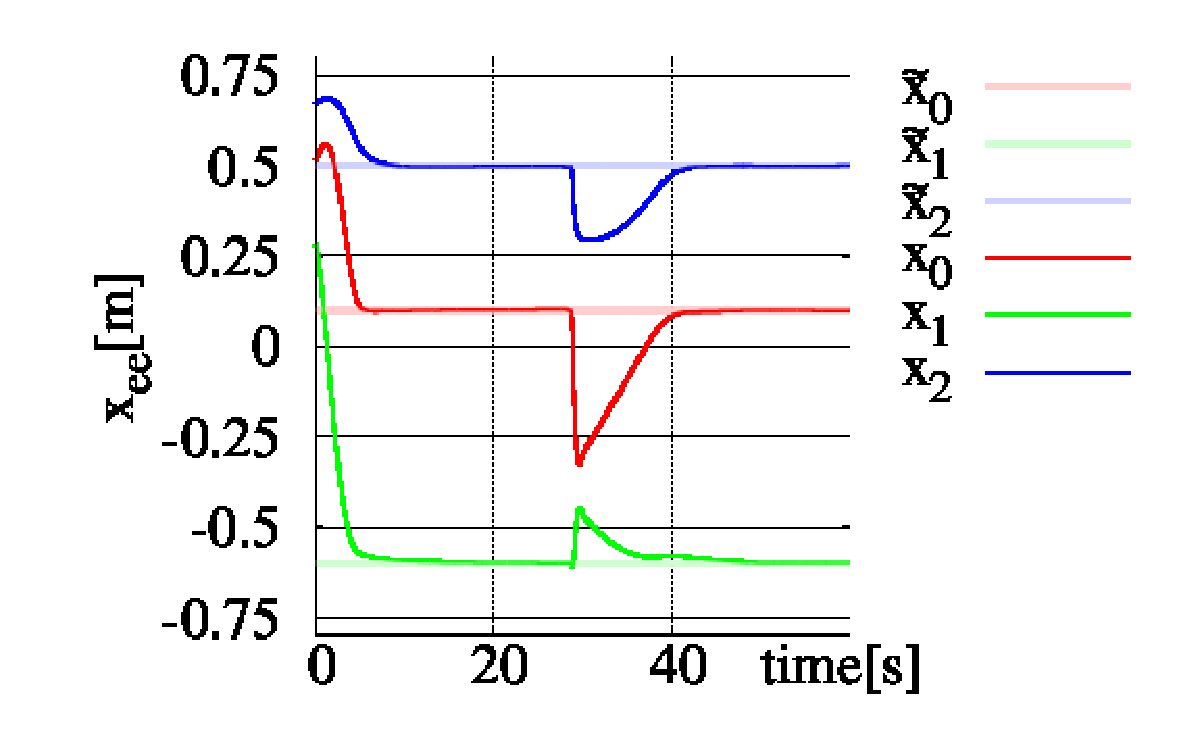
\includegraphics[width=1.\textwidth]{3_moving_obstacles/realPanda/trajectory_static}
    \caption{Static Fabric}%
    \label{subfig:experiment3_realPanda_trajectory_static}
  \end{subfigure}%
  \begin{subfigure}{0.5\linewidth}
    \centering
    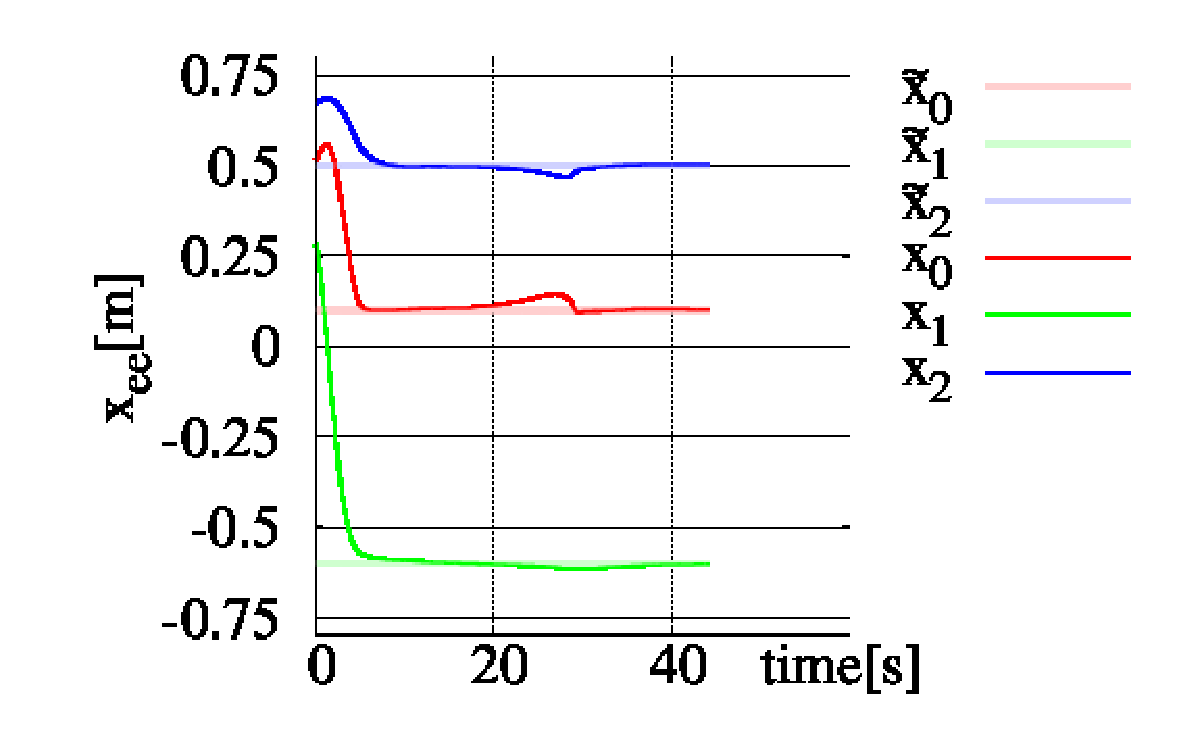
\includegraphics[width=1.\textwidth]{3_moving_obstacles/realPanda/trajectory_dynamic}
    \caption{Dynamic Fabric}%
    \label{subfig:experiment3_realPanda_trajectory_dynamic}
  \end{subfigure}
  \caption{Trajectories for real panda robot in the presence of a dynamic obstacle. \ac{df}
    show a smoother and in-advance reaction to the approaching obstacle
    while \ac{sf} can only react in sudden motion.
  }%
  \label{fig:experiment3_realPanda_example}
\end{figure}

\iffalse%
\MS{Takeaway Experiment3: Only dynamic fabrics are able to respect dynamic obstacles.}
\fi


